% !TEX root = ./First_year_report.tex

\chapter{Quantum Computing}
 
At a fundamental level, quantum computing is a discipline focused on developing hardware and software frameworks that leverage quantum mechanics to solve difficult problems. Whereas a classical computer uses information encrypted in elements called bits, taking values of 0 and 1, quantum computer elements can be in a superposition of states, and experience phenomena such as entanglement. The goal is to use quantum systems to solve computationally demanding problems more efficiently than the most powerful conventional computers. 

It is also worth mentioning that the work needed to achieve this has and will likely continue to contribute to our understanding of quantum mechanics and the development of new techniques in superconductivity, control of quantum systems and more. Due to this, progress in the field is important beyond short- or intermediate-term applications.

This chapter introduces the basic concepts behind quantum computing and provides a brief overview of the current state of the field. Afterward, the focus is on Quantum Error Correction, one of the main challenges behind this technology. Due to the nature of this project, the topics will be introduced from the well-known qubit-based perspective alongside the bosonic (quantum resonator-based) architectures.

\section{Fundamentals}
\subsection{The qubit and superposition}

The building block of quantum computation is known as the qubit or quantum bit. This concept is analogous to the more familiar bit, the smallest binary element in a classical computer. To establish a quantum information framework, the qubit can be defined in abstract terms as a two-level quantum system with possible states $\ket{0}$ and $\ket{1}$. This is an apt description of a variety of physical elements that can be used to build real computing systems, such as electron spins, photon polarization or superconducting circuits.

Due to its quantum mechanical nature, state $\ket{\psi}$ of a qubit is expressed as a superposition (linear combination) of states $\ket{0}$ and $\ket{1}$ as follows:
\begin{equation}
    \ket{\psi}=\alpha\ket{0}+\beta\ket{1}.
\end{equation}
Amplitudes $\alpha$ and $\beta$ are complex numbers obeying $|\alpha|^2+|\beta|^2 = 1$. It is possible to observe a bit and determine that its state is 0 or 1. In the case of a qubit in a superposition, an examination of its state gives less complete information. The outcome of the measurement will be $\ket{0}$ with probability $|\alpha|^2$ and $\ket{1}$ with probability $|\beta|^2$. Note that the properties of $\alpha$ and $\beta$ ensure that the probabilities of the states add up to unity.

The length 1 qubit states can be represented in a Block sphere, parametrizing the whole continuum of qubit states.
\begin{figure}
    \centering
    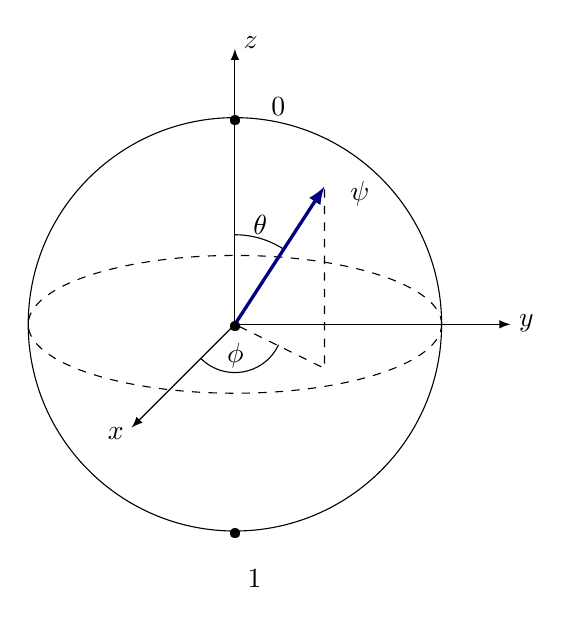
\begin{tikzpicture}[scale=1.75]
        \draw (0,0) circle (1.5);
        \draw[dashed] (0,0) ellipse (1.5 and 0.5);
        \draw[-latex] (0,0)--(2,0) node[label={[shift={(0.2,-0.35)}]$y$}]{};
        \draw[-latex] (0,0)--(0,2) node[label={[shift={(0.2,-0.25)}]$z$}]{};
        \draw[-latex] (0,0)--(-0.75,-0.75)node[label={[shift={(-0.2,-0.4)}]$x$}]{};
        \node[label={[shift={(0.55,-0.25)}]$\ket{0}$}] at (0,1.475){\textbullet};
        \node[label={[shift={(0.25,-1)}]$\ket{1}$}] at (0,-1.525){\textbullet};
        \draw[rotate=90] (0.65,0) arc (0:-33:0.65) node[midway,label={[shift={(0,-0.2)}]$\theta$}]{};
        \draw[-latex,NavyBlue,very thick] (0,0)--(0.65,1);
        \node at (0,-0.025){\textbullet};
        \draw[dashed](0.65,0.98)--++(0,-1.3)--(0,0);
        \node[label={[shift={(0.45,-0.5)}]$\ket{\psi}$}] at (0.65,1){};
        \draw[rotate=-135] (0.35,0) arc (0:110:0.35) node[midway,label={[shift={(-0.1,-0.2)}]$\phi$}]{};

    \end{tikzpicture}
    \caption[Bloch sphere representation of a qubit state]{Bloch sphere representation of an arbitrary qubit state (blue). Note how the orthogonal basis states $\ket{0}$ and $\ket{1}$ are shown as diametrically opposite.}
    \label{fig:bloch_sphere}
    \end{figure}
In the Bloch sphere, qubit states are represented in three-dimensional space in terms of two real parameters $\theta$ and $\phi$:
\begin{equation}
    \ket{\psi} =\cos \left(\theta /2\right)\ket{0} \,+\,e^{i\phi }\sin \left(\theta /2\right)\ket{1},
\end{equation}
with $0\leq \theta \leq \pi$ and $0\leq \phi \leq 2\pi$. Although at first glance it would appear there is an infinite amount of states that can be represented within a qubit. This however doesn't imply that an infinite amount of information can be encoded within it. Due to the quantum measurement phenomenon known as state \textit{collapse}, the outcome of qubit measurement will be either 0 or 1, providing one bit's worth of information. In fact, an exact determination of the parameters in a qubit state would require measuring an infinite number of identical qubits. At the same time, the properties of unmeasured qubits are essential to the power of quantum processing.

\subsection{Composite systems and entanglement}

Much in the same way as in classical computation, to carry out useful computations, several information units are needed. Therefore, it is essential to discuss how different qubits will interact with each other. When introducing a second qubit, the set of basis states will contain four elements, spanning all state combinations for both qubits: $\ket{00}$, $\ket{01}$, $\ket{10}$, and $\ket{11}$. The general state of the two-qubit system can be expressed as a superposition of the basis states, given by four complex amplitudes.
\begin{equation}
    \ket{\psi} = \alpha_{00}\ \ket{00}\ +\ \alpha_{01}\ \ket{01}\ + \ \alpha_{10}\ \ket{10}\ +\ \alpha_{11}\ \ket{11}
\end{equation}
Once more the squared norms of the amplitudes will represent the probability of measuring each state. Consequently, the state must be normalized according to $\sum_i |\alpha_i|^2 = 1$, for $i$ spanning all basis states. A measurement of this system could be applied to only one of the qubits, with a post-measurement superposition state conditioned on this outcome. For example, the first qubit will be measured at state $\ket{0}$ with probability $|\alpha_{00}|^2 + |\alpha_{01}|^2$. After obtaining this result, the system will be left in a normalized superposition of states $\ket{00}$ and $\ket{01}$.

An essential quantum behaviour that emerges when working with multiple qubits is the entanglement property, as best illustrated by Bell states (also known as Einstein-Podolsky-Rosen pairs). Consider the following superposition:
\begin{equation}
    \psi = \cfrac{\ket{00}\ +\ \ket{11}}{\sqrt{2}}.
\end{equation}
If the first qubit in this composite state is measured, the outcome will be $\ket{0}$ or $\ket{1}$ with respective probabilities of $1/2$. What is most interesting is what our measurement tells us about the state of the system overall. If the first qubit is in state $\ket{0}$ ($\ket{1}$), after measurement the system must be in state $\ket{00}$ ($\ket{11}$). Therefore, there is only one possible state the second qubit is allowed to be in, and gaining this information did not require performing a direct measurement. This shows how quantum elements can be correlated beyond what is possible for a purely classical system, and this property will be the basis of useful methods within the discipline of quantum computing. 

While discussing multi-qubit systems it is worth noting that for an $n$-state system, the basis states are simply a generalization of what has been discussed for the two-qubit case. It will once again be given by all possible combinations of qubit states. As a consequence the total number of encoded states grows quickly as $2^n$, achieving very high state numbers with qubit numbers in the hundreds. Due to the probabilistic nature of the qubits, it is possible to work with large amounts of quantum numbers simultaneously, far beyond what can be encoded classically.

So far, this section has focused on qubits as the essential units for quantum information. For the purpose of computation, however, the information must be manipulated as per the end goal. The next subsection discusses the gate operations that make this possible.


\subsection{Quantum logic gates}

In order to perform computations, bits and qubits, are used as part of computer circuits, in which information gets converted and transmitted. The operations to be applied can be as simple as the classical $NOT$ gate, which flips the value of a bit. If the bit is in state 0 it is changed to state 1, and vice versa. Logic gates can of course be more elaborate, for example, taking into account more than one bit.

Naturally, one must think of what gates must look like in quantum computers, taking into account knowledge of qubit states and quantum mechanics. The first key difference between a bit and a qubit is that the latter involves a linear combination of basis states. Therefore, a quantum logic gate needs to be able to act on this superposition state. To be compatible with quantum mechanics, and maintain the sense of probability, a quantum $NOT$ gate needs to be a linear operation.

Quantum logic gates are commonly expressed as matrices in the state basis. For the quantum $NOT$ case, the matrix representation is:
\begin{equation}
    X \equiv \begin{bmatrix}
    0&1\\
    1&0
    \end{bmatrix},
\end{equation}
where the first column and row correspond to state $\ket{0}$ and the second to state $\ket{1}$. Likewise, the qubit state can be represented as a vector in this basis:
\begin{equation}
    \ket{\psi}=\begin{bmatrix}
    \alpha\\
    \beta
    \end{bmatrix}.
\end{equation}
Then the quantum $NOT$ gate acts on the qubit as:
\begin{equation}
    X\ket{\psi} = \begin{bmatrix}
        \beta\\
        \alpha
        \end{bmatrix},
\end{equation}
flipping the amplitudes associated with each basis state.

Linearity is not the only property of quantum mechanical systems that must be reflected in quantum logical gates. As was mentioned previously, the probabilistic nature of qubits requires states to be normalized. This must be true before and after a logic operation is applied to the qubit (probability must be conserved). Therefore, any $2\times 2$ matrix $U$ associated with a quantum gate must be unitary, obeying
\begin{equation}
    U^\dagger U = I,
\end{equation}
where $I$ is the $2\times 2$ identity operator.

The properties of linearity and unitarity generalize for gates acting on multiple qubits. One useful example of this is the two-qubit CNOT gate (also known as controlled $NOT$):
\begin{equation}
    CNOT=\begin{bmatrix}
        1&0&0&0\\
        0&1&0&0\\		 		
        0&0&0&1\\
        0&0&1&0\\
    \end{bmatrix}
\end{equation}
This gate performs a $NOT$ operation on the second qubit, as conditioned by the state of the first qubit (which is left unchanged). The effect of this gate is summarized in the following table:

\FloatBarrier

The equivalency between the $CNOT$ gate and a classical counterpart is not as direct as what can be drawn between the classical and quantum $NOT$ operations. This is due to yet another useful property stemming from the quantum nature. Quantum logical gate representations are always invertible, meaning that their effect is reversible. Meanwhile, the classical analogue to the $CNOT$ operation ($XOR$ gate) loses information, and therefore the state before its application cannot be recovered.

 It is worth mentioning as well that the conditional action based on the state of the first qubit does not constitute a measurement. Due to this, it does not cause a collapse of the superposition state, making the $CNOT$ gate an extremely powerful tool. In fact, it is proven that the use of $CNOT$ gates alongside the set of single-qubit rotations is sufficient to perform any operation (on any number of qubits). This is known as universality, and can theoretically be realized to arbitrary accuracy.
 Another aspect of note is that the $CNOT$ gate can be used to prepare entangled states, such as the aforementioned Bell states.

\section{Current Capabilities}

\subsection{The NISQ era}
Presently, quantum computing is in its NISQ era, standing for (Noisy Intermediate-Scale Quantum). This denomination refers to some of the main challenges of quantum computation. 

The first challenge is noise. Even within the context of classical computing, there exists a possibility of random errors that may modify the state of one or more bits. The quantum properties of qubits make them particularly susceptible to environmental interference. As was discussed previously, an interaction (or measurement) will lead to quantum decoherence, and so eliminate the useful characteristics of the system. Due to this, hardware implementations need to put special emphasis on, for example, isolating qubits and preventing thermal fluctuations. 

Another way of approaching noise mitigation is implementing error correction algorithms, which can identify and rectify issues that arise. Executing these algorithms, however, necessitates using more qubits in a given calculation. This leads to the second challenge of the NISQ era: the intermediate scale. This refers to the size of the quantum systems that can actually be realized in hardware. The size or volume is thought of in terms of qubit number and number of applied gates. In a circuit comprised of qubits with some probability of failure, the probability of having some error increases with the qubit number. Likewise, whenever a gate is applied there is some probability an error will be caused, so the overall probability of error increases the more we operate on the system.

Recent work by several companies (such as IBM, Rigetti, and Google) has enabled great strides in the number of qubits of current quantum systems, which in the last few years has jumped from below 50 to around 1000 qubits. In the short and intermediate term, there is still plenty of work to be done to not only allow for the increase of this number, but also ensure higher coherence times, more accurate gate operations, and more efficient error correction algorithms. These are some of the elements that will come into play in the development of fault-tolerant\footnote{Fault tolerant systems can continue functioning adequately even if some errors or partial failures are present.} quantum computers and the achievement of quantum advantage\footnote{Quantum advantage refers to conclusively proving that a quantum computer can solve a problem that no classical computer can solve within a reasonable timeframe. Computationally complex problems can often be theoretically computable classically, however, due to exponentially increasing timeframes may only be achieved at time scales beyond human interest.}.

The basic ideas behind Quantum Error Correction, along with some examples, will be addressed in a later chapter. The next subsection provides an overview of some of the physical systems that are currently used as quantum hardware.

\subsection{Hardware approaches}

As was described in the previous subsection, the quantum computing framework can be carried out through different physical systems. These include, for example, superconducting qubits, trapped ions, and photonics. The following descriptions do not aim to provide a comprehensive overview of each hardware architecture, and instead hope to provide a more grounded idea of how quantum computing is carried out. As will be described, each hardware implementation presents a set of limitations that need to be addressed to develop usable quantum computers. At the same time, each of them can also provide unique advantages and can be worked with from different conceptual points of view. 

Perhaps the best-known type of quantum hardware is based on superconducting qubits. These systems build qubits from Josephson junctions, formed by two superconducting elements separated by a fine insulator layer. Due to the Josephson effect, this junction will allow a current between the superconductors, enabled by \textit{quantum tunnelling}\footnote{Quantum tunnelling is a quantum mechanical effect that allows particles to go through barriers (such as the walls of a potential well), despite their energy being lower than that needed to surmount them according to classical physics.}, thus displaying a quantum effect at a macroscopic scale. The logical qubit states $\ket{0}$ and $\ket{1}$ can be mapped to different physical states of the superconducting components, such as discrete energy levels. The elements are then arranged into a circuit. 

In order to manipulate these superconducting circuits to perform computations it is necessary to construct reliable control operations. In the case of superconducting qubits, microwave pulses can be administered to execute single-qubit or multiple-qubit gate operations. The control and readout of the superconducting qubits are carried out using classical computers, that are already built for user interfacing.

Due to their superconducting nature, these systems need to be maintained at cryogenic temperatures to prevent decoherence. The cabling linking circuit elements and aspects such as qubit readout also need to be optimized to minimize incidences of errors and allow for the scalability of the systems. In other words, technical advances in hardware development are essential to building quantum computers with larger qubit numbers that can execute more gate operations, while avoiding the exponential increase of errors. Some of the companies focused on this task are Rigetti, IBM, and Google.

Computation using superconducting qubits does not always rely on gate operations. This is the case in quantum annealers, such as those developed by D-wave. These systems apply magnetic fields to superconducting qubits that can manipulate the probability of a qubit being in each state (bias). Lattice configurations are assembled for these qubits, establishing couplings between them with arbitrary correlation weights. A user choice of qubit biases and couplings can be used to solve optimization-type problems. The annealing process consists of slowly evolving the system from a ground state of unbiased and uncorrelated qubits into the ground state of the problem that the user desires to solve.

A classic case of an optimization problem is that of the travelling salesman. The goal of the problem is to find the shortest route for the traveller between a set of towns. Although coming up with a classical algorithm to solve this problem is straightforward (simply calculate distances for all possible paths and compare), its computational cost increases exponentially with the number of towns. Thus, the problem cannot be solved by classical computers for non-trivial cases (although heuristic solutions exist that provide approximate solutions for some more complex cases).

This is the type of problem that could benefit from a quantum annealing-based computer. In this case, the correlations between qubits represent the distances between the cities. Meanwhile, the qubit states contain the information on whether a town was (or wasn't) visited in a sequence step. The total system energy for a given state is associated with the distance traversed by the traveller if the towns were visited in that particular order. Thus, the ground state provided by an annealer will correspond to the desired solution, the optimal path. It is worth noting that this approach is also liable to qubit decoherence, as well as other sources of error. Furthermore, the annealing process can be heuristically transposed into gate-based quantum computers to address optimization problems.

A third type of quantum computer is the bosonic system. This dispenses with the focus on two-level qubits. Instead, bosonic computing's basic unit is the qudit, which can have N levels. In physical terms, a qudit is implemented using a quantum harmonic oscillator, and assigning a logical state to each of its accessible energy levels. Quantum oscillator systems can be built using Superconducting radio-frequency (SRF) cavities, which have very low rates of dissipation and are therefore well equipped to maintain state coherence. 

The ability to encode a higher number of states within one single hardware element is key to implementing Quantum Error Correction procedures without introducing new sources of noise. The possible errors in a resonant cavity are linked to photon loss, which is easy to detect and correct. These advantages have turned bosonic platforms into an area of high interest and expectation. As bosonic quantum computing is a focus of this PhD, a further section will be dedicated entirely to this particular topic.





\vspace{5cm}
Qubits, NISQ overview: \cite{Nielsen2010} \cite{Preskill2018} \cite{IBMintro} \cite{Kaye2007} \cite{Cleve2021}. 
Expected applications (brief), perhaps better suited to the intro section?

Different hardware approaches (brief): \cite{Dwave} \cite{Zurich} \cite{IBMtec}

Bosonic systems: \cite{Zurich} \cite{Girvin2021}, cQED

\clearpage
\chapter{Quantum Error Correction}

As was established in prior sections, quantum computers are susceptible to environmental noise which jeopardizes the coherent states containing information. The field of error correction is well-established for classical computers. However, classical corrections algorithms cannot simply be applied to quantum systems. Qubits, unlike bits, are limited by the no-cloning theorem, stating that it is not possible to make independent, perfect copies of a qubit's state. There is also the problem of quantum measurement and wavefunction collapse. Despite this, Quantum Error Correction (QEC) is a productive field of study, and many viable approaches to error mitigation have been proposed. The following section aims to introduce the fundamental ideas behind QEC at the qubit level and the bosonic level, alongside some example implementations.

\section{Introduction to Error Correction}

One of the basic ideas behind error correction is that of redundancy. In simple terms, it consists of using a higher number of bits (or qubits) to encode one bit (or qubit) of information. A simple illustrative example is that of the classical repetition code. Instead of just utilizing one bit with possible values of 0 and 1, one can define logical codewords. These logical codewords are strings of multiple bits, mapped to logical states 0 and 1. For the three-bit repetition code, codeword '000' (three bits in state 0) corresponds to logical state 0, while codeword '111' does to logical 1. 

In classical computing, there is only one possible error, known as bit flip. A bit flip occurs when a bit in 0 gets mapped to 1, or vice versa. When transmitting the logical states, the receiver could get '100', '010' or '001' instead of codeword 0, assuming only one bit flip occurs. This error can easily be remedied using \textit{majority voting}. Simply put, if most of the bits take value 0, the 1-valued bits are assumed to have flipped, and the error can be rectified. 

If two bits happen to flip, the error can be detected, as the transmitted bit string does not match either codeword. However, this error cannot be corrected using majority voting, and the received logical bit will be incorrect. If three errors occur, the situation is even more dire, as the resulting state is still a valid codeword, and the error cannot be detected, much less rectified. This does not mean that the three-bit repetition code (despite being inefficient) is unable to provide any improvement. Error correction is based on the assumption that hardware performs well enough that errors are rare. Thus the goal is not to provide ideal error correction but to further reduce the already low incidence of errors. In the case of the three-bit repetition code, low error probabilities mean that uncorrectable errors (two or three bit-flips) are significantly less likely than the correctable single bit-flip. Likewise, undetectable errors are the least likely to occur. 

It is worth noting that some tools to address errors can be designed with only detection (and not correction) in mind. For example, for an arbitrary bit string, an additional bit can be implemented to record the string (plus ancilla) parity. This is achieved by mapping even and odd parity to 0 and 1. If at a later stage the parity of the new bit string is odd, an odd number of bit-flips must have occurred. The exact details of the errors cannot be obtained from the bit string, but the string is known to be corrupted. Given that the incidence of no-flip and one bit-flip events is much higher than that of two bit-flips (where parity is indistinguishable from the errorless case), it is reasonable to assume that an even parity implies that no bit has flipped. Likewise, it is to be expected that an odd parity was caused by one single error.

When adding ancilla bits, it is important to consider that the error rate is a priori increased. Consider once again the repetition code. If each bit in a certain hardware system is known to have a probability of error $\epsilon$, the probability of having no errors on a bit is: \begin{equation}
    P_0=1-\epsilon.
\end{equation}.
Once the ancillae are introduced, this becomes:
\begin{equation}
    P_0=(1-\epsilon)^3.
\end{equation} 
Therefore, the probability of at least one error occurring is 
\begin{equation}
    1-P_0 \sim 3\epsilon,
\end{equation} 
tripling that of the single bit (in the small $\epsilon$ limit). Thus, a successful error correction code must surpass the break-even point: the logical (error-corrected) bit error rate must be lower than for the physical bit. 

Consider the break-even point for the repetition code. The logical bit error rate is given by the probability of running into an uncorrectable error (having two or three bit-flips). This can be expressed as:
\begin{equation}
    \epsilon_{logical} = P_2 + P_3 = 3\epsilon^2 - 2\epsilon^3.
\end{equation}
Probabilities $P_2$ and $P_3$ correspond to the two and three-bit-flip cases respectively. For this case their values are $P_2 = 3\epsilon^2(1-\epsilon)$ and $P_3 = \epsilon^3$.

The breakeven point equation $\epsilon_{logical}=\epsilon$ shows that the repetition code will reduce error occurrences for physical bit error rates below $1/2$. For error rates above this, the code application will in actuality be detrimental. The form of $\epsilon_{logical}$ also shows that, as expected, logical bit error rates decrease with physical bit error rates.

It is worth noting that introducing error correction for bit flips does not provide complete fault tolerance, as more realistic error models need to take into account errors introduced when other system elements fail. This includes accounting for possible errors in the error-correction circuitry itself or errors attributed to the process of measuring bit states. For example, a realistic logic gate will have some chance of failing when used. The goal is to design error correction circuits that only incur errors that it can detect and correct in its subsequent applications.
This also affects the frequency at which the correction process must be applied.

If there is a certain probability of each bit in the system flipping in a given time interval, a repetition-code-based correction scheme needs to be applied before the probability of uncorrectable errors becomes too large. However, if the correction code is applied too often, there is a risk of having error correction circuit errors (such as incorrect majority voting). Near-perfect correction circuits should enable fault tolerance through speedy circuit implementations. However, realistically, the delay between operations will be affected by the take to execute.

Having discussed some of the basic concepts and motivations when performing error correction, let us move on to applications to qubit-based systems.


\section{Error correction for qubit systems}

As was described in the first section, qubit states exist within the continuum of all states in the Bloch sphere. Consequently, a clear difference between bit and qubit errors will stem from the multiplicity of error types in the latter case. A qubit can experience coherent errors taking it into any other of the infinite possible states, rather than just being shifted from 0 to 1.

A coherent error acting on a qubit can be expressed in terms of a unitary operation\footnote{An error could also be non-unitary due to entanglement with a bath and wavefunction collapse.}, just like quantum logical gates. The unitary operator $U(\delta\theta,\delta\phi)$ represents the evolution of the quantum state as it shifts to coordinates $\theta+\delta\theta$ and $\phi+\delta\phi$ in the Bloch sphere space. It can be expressed mathematically as:
\begin{equation}
    U(\delta\theta,\delta\phi)\ket{\psi} = \cos\frac{\theta+\delta\theta}{2}\ket{0}+e^{i(\phi+\delta\phi)}\sin\frac{\theta+\delta\theta}{2}\ket{1}.
\end{equation}

At first glance, it would seem impossible to address all the arbitrary errors that could take place in any given qubit. However, the problem is simplified by considering that the error operator can be expressed as an expansion in the Pauli basis. For two-dimensional matrices this is given by:
\begin{equation}
    I=\begin{bmatrix}
        1&0\\
        0&1
    \end{bmatrix},\quad
    X=\begin{bmatrix}
        0&1\\
        1&0
    \end{bmatrix}, \quad
    Y=\begin{bmatrix}
        0&-i\\
        i&0
    \end{bmatrix},\quad
    Z=\begin{bmatrix}
        1&0\\
        0&-1
    \end{bmatrix}.
\end{equation}
Then, the single-qubit error operation can be expanded as:
\begin{equation}
    U(\delta\theta,\delta\phi)\ket{\psi}=\alpha_I I\ket{\psi} + \alpha_X X\ket{\psi} + \alpha_Y Y\ket{\psi} + \alpha_Z Z\ket{\psi},
\end{equation}
for $\alpha_i$ representing expansion coefficients. This way, any coherent error can be decomposed as a combination of four operations. The ability to correct Pauli-X and Pauli-Z errors will be enough to perform any correction. This is because Pauli Y can be expressed as $Y=XZ$. 

An error described by Pauli matrix $X$ is analogous to a classical bit-flip error. Its action on the generic qubit state is:
\begin{equation}
    X\ket{\psi}=\alpha X\ket{0}+\beta X\ket{1} = \alpha \ket{1}+\beta \ket{0}.
\end{equation}
On the other hand, an error caused by the Z matrix is known as a phase-flip error and has no classical equivalent. The operation leaves the $\ket{0}$ state unchanged, while mapping state $\ket{1}$ to $-\ket{1}$. The effect on an arbitrary qubit state is as follows:
\begin{equation}
    Z\ket{\psi}=\alpha Z\ket{0}+\beta Z\ket{1} = \alpha \ket{0} -\beta \ket{1}.
\end{equation}
This is equivalent to a $180^\circ$ rotation around the $z$-axis on the Block sphere shown in Figure \ref{fig:bloch_sphere}.

As was mentioned previously, there is a key difference between classical and quantum error correction, beyond the introduction of the phase-flip. Due to the no-cloning theorem, quantum error correction codes cannot rely on making perfect copies of the qubit state. For the repetition code example, it was shown that the physical bit state was applied to two ancilla bits to form logical codewords '000' and '111'. This cannot be replicated for a qubit. A further limitation stems from the wavefunction collapse that can be triggered when a state measurement is applied. Thus, QEC constitutes a framework going beyond the tools of classical computing, as will be subsequently shown.

\subsection{A simple two-qubit code}

Let us now begin to visualize the strategies of QEC through an elementary example. The goal of the code is to detect bit flips on a single qubit. As in the classical case, it is necessary to increase the amount of information that is being stored, beyond that contained on the qubit. Consider the introduction of a second qubit. In order to provide redundancy, this ancillary qubit must reflect the state of the first one. However, as discussed, it is not possible to simply make a copy of the initial qubit or measure it and obtain complete state information. Logical states can be obtained by an encoding procedure entangling the qubits, with the following outcome:
\begin{equation}
    \ket{\psi}= \alpha \ket{0} +\beta \ket{1} \quad \rightarrow \quad \ket{\psi}_L = \alpha \ket{00} +\beta \ket{11}=\alpha \ket{0}_L +\beta \ket{1}_L
\end{equation}
The encoding is straightforward to achieve by implementing a CNOT gate as shown in Figure \ref{fig:two_qub_enc}, requiring no knowledge of the qubit state.

\begin{figure}
    \centering
    \begin{tikzpicture}
    \node[scale=1.25] {
    \begin{quantikz}
        \lstick{$\scriptstyle\ket{\psi}$} & \ctrl{1} & \rstick[2]{$\scriptstyle\ket{\psi}_L$}\\
        \lstick{$\scriptstyle\ket{0}$}& \targ{} &
    \end{quantikz}};
    \end{tikzpicture}
    \caption{CNOT gate encoding circuit to implement two-qubit bit-flip detection.}
    \label{fig:two_qub_enc}
\end{figure}
Qubit state information has now been distributed into the 4-dimensional Hilbert space spanning states $\ket{00}$, $\ket{01}$, $\ket{10}$, and $\ket{11}$. The subset of Hilbert space comprised by $\ket{00}$ and $\ket{11}$ is known as \textit{codespace}, and it corresponds to the non-bit-flipped states. If the logical state experiences a bit-flip error, such as
\begin{equation}
    X_1\ket{\psi}_L = \alpha\ket{10} + \beta\ket{01}
\end{equation}
for $X_1$ representing a flip on the first qubit, it will be rotated into the \textit{error} subspace. Error space is orthogonal to codespace. Due to this, projective measurements can be carried out to distinguish between error space and codespace states without compromising qubit encoding. The projective measurements used to identify the bit flips are known as \textit{stabilizers}. The term references the fact that these operations leave logical states unchanged. 

In this case, the stabilizer operation is $Z_1Z_2$, where $Z_1$ and $Z_2$ refer to Pauli Z operations on qubits 1 and 2, respectively. This is essentially a generalization of the $Z$ gate to the logical state (rather than a single qubit). It is straightforward to verify that the logical state $\ket{\psi}_L$ is an eigenstate of the stabilizer with eigenvalue $+1$. Meanwhile, bit flipped states $X_1\ket{\psi}_L$ $X_1\ket{\psi}_L$ are eigenvalue $-1$ eigenstates of $Z_1Z_2$. The operation is essentially a joint parity operation, identifying whether both qubits are in the same state. Therefore, these outcomes can be used to distinguish between codespace states and erroneous states without compromising the information given by the $\alpha$ and $\beta$ superposition parameters. The resulting classical information provided by the stabilizer measurement is known as \textit{error syndrome}. A limitation of this code is that the exact nature of the error that occurred is not revealed by the syndrome. That is, it is not possible to distinguish between the $X_1$ error (bit-flip on qubit 1) and the $X_2$ error (bit-flip on qubit 2). Consequently, there is not enough information to perform an error correction (by re-applying the appropriate error operation). In order to do this, a three-qubit generalization of the code must be implemented.

\subsection{The three-qubit code}

The setup for the three-qubit code consists of entangling the qubit state in need of preserving with two ancilliary qubits. The process is very similar to that for the two-qubit code, now involving two CNOT gates, as shown in Figure \ref{fig:three_qub_enc}.
\begin{figure}
    \centering
    \begin{tikzpicture}
    \node[scale=1.25] {
    \begin{quantikz}
        \lstick{$\scriptstyle\ket{\psi}$} & \ctrl{1} & \ctrl{2} & \rstick[3]{$\scriptstyle\ket{\psi}_L$}\\
        \lstick{$\scriptstyle\ket{0}$}& \targ{} & &\\
        \lstick{$\scriptstyle\ket{0}$}& & \targ{} & 
    \end{quantikz}};
    \end{tikzpicture}
    \caption{CNOT gate encoding circuit to implement three-qubit bit-flip detection.}
    \label{fig:three_qub_enc}
\end{figure}
The encoding results in the logical state
\begin{equation}
    \ket{\psi}_L = \alpha \ket{000} +\beta \ket{111}=\alpha \ket{0}_L +\beta \ket{1}_L.
\end{equation}

Consider once again that the only possible errors are bit-flips. Then there are three error operators, representing a flip on each qubit: $X_1$, $X_2$, and $X_3$. Error checks can now be performed with a set of two stabilizers: $S_1=Z_1Z_2$ and $S_2=Z_2Z_3$\footnote{Once again the indices refer to the operations acting on different qubits.}. The pair of operators commute, obeying $\left[S_1,S_2\right]=S_1S_2-S_2S_1=0$. This implies that both stabilizer measurements can be performed simultaneously. As in the two-qubit code, the codespace states are eigenstates of the operators with eigenvalues of $+1$. The stabilizers also commute with the set of logical state operators:
\begin{eqnarray}
    X_L&=X_1X_2X_3 \\
    Y_L&=-iX_LZ_L=-Y_1Y_2Y_3\\
    Z_L&=Z_1Z_2Z_3
\end{eqnarray}
As a result, it is concluded once again that applying the stabilizer measurements does not affect the coherence of the logical state.

Measuring the two stabilizer provides two bits of information, which is sufficient to identify the error type. If the error is identified, then the appropriate error operation can be applied to revert it. Once again, the stabilizers constitute parity operations, and thus can identify whether or not a pair of qubits are in the same state. In this case, different combinations of the measured syndromes can be related to a particular bit flipping. The different syndromes are shown in the following table:
\begin{table}[hbt!]
    \centering
    \begin{tabular}{ l || c | c}
        Error & $S_1$ & $S_2$ \\ 
         \hline \hline
         $I$ & $+1$ & $+1$ \\ 
         $X_1$ & $-1$ & $+1$\\ 
         $X_2$ & $-1$ & $-1$\\
         $X_3$ & $+1$ & $-1$
    \end{tabular}
\caption[Error syndrome outcomes for stabilizers in the three-qubit code]{Error syndrome outcomes for stabilizers $S_1$ and $S_2$ as linked to each possible error ($I$ represents the no error case)}
\end{table}

It is possible to define a third stabilizer $S_3=Z_1Z_3$. This is equivalent to the product of the other two stabilizer, and as such does not provide any new information. However, it could be useful to find errors in the stabilizer measurement process.

The two examples provided provide very simple (but not necessarily practical) introductions to what quantum error correction looks like. In reality, more complex codes need to be implemented to address errors more efficiently, as well as addressing errors such as phase flips and entanglements with a bath. Following is a discussion of the tools that can be applied to determine if a code is capable of error correction.

This behaviour of this code was tested and visualized by implementing it using Python. Although quantum computing packages such as Qiskit are available, a more hands-on approach was taken, coding the linear algebra involved in the process. As a result, we visualized how the probability of a bit-flip occurring affects the success rate of the code over several tests (that is, how often the error correction execution managed to preserve the qubit state). This result is shown on Figure \ref{fig:three-qbit-code-success}.
\begin{figure}
    \centering
    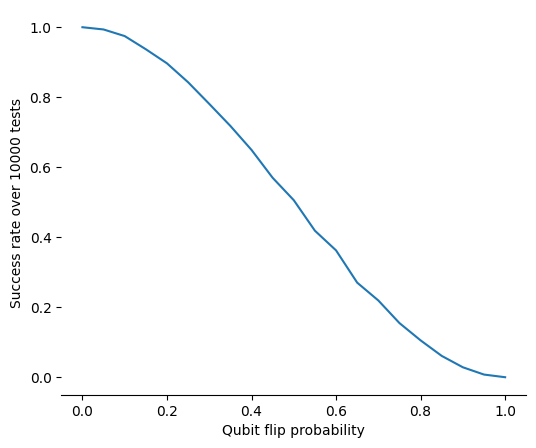
\includegraphics[scale=0.6]{Success_rate.png}
    \caption{Success rate of the three-qubit error correction code for different bit-flip probabilities.}
    \label{fig:three-qbit-code-success}
\end{figure}

\section{Error Correction and the Knill-Laflamme Conditions}

An often useful tool to work with quantum states comes from the density matrix formulation. The state of a quantum system can be expressed as an operator taking the following form:
\begin{equation}
    \Hat{\rho} = \sum_j p_j \ket{\psi_j}\bra{\psi_j}.
    \label{eq:dens_mat}
\end{equation}
This represents a mixture of states, each occurring with some probability given by $p_j$ (naturally this must obey $\sum_j p_j = 1$). States $\ket{\psi_j}$ are known as pure states. In previous sections, the qubits were assumed to be in some determined (pure) superposition state. However, when a quantum system experiences entanglement with a bath, the bath state is inaccessible. Given the knowable information, the system could be in any one of some set of pure states, and its full description is given by the statistical mixture in equation \ref{eq:dens_mat}\footnote{If $p_i=1$ and $p_j=0 \;\forall\ j \neq i$ the density matrix corresponds to a pure state $\Hat{\rho} = \ket{\psi_i}\bra{\psi_i}$, and the matrix is a projection.}. Then, the system is said to be in a mixed state. By being able to represent both pure and mixed states, the density matrix provides a general approach to computing expectation values for a quantum operation. 

The Hermitian density matrix has a few key properties: 
\begin{itemize}
    \item Unit trace: $\mathrm{Tr}\left[\hat{\rho}\right] =\sum_j p_j = 1 $
    \item Semi-positive-definite: $\bra{\psi}\hat\rho\ket{\psi}\geq 0$
    
    Therefore the matrix has only real and non-negative eigenvalues.
    \item If (and only if) the represented state is pure:
    \begin{itemize}
        \item $\hat\rho=\hat\rho^2$
        \item $\mathrm{Tr}\left[\hat\rho^2\right] = 1$.
    \end{itemize}
\end{itemize}

Both unitary state evolutions (such as a bit-flip error) and those due to non-unitary operators (bath entanglement) must preserve these properties. These transformations are known as CPTP maps, standing for Completely-positive Trace-preserving. The evolution of the density matrix under CPTP maps during time interval $\Delta t$ can be expressed using the \textit{Kraus representation}:
\begin{equation}
    \hat\rho'=\hat\rho(t+\Delta t)= \sum_\ell \hat K_\ell \hat\rho(t) \hat K_\ell^\dagger,
    \label{eq:kraus_rep}
\end{equation}
where $K_\ell$ are Kraus operators. The set of Kraus operators $\mathcal{E}=\{ K_0,K_1,K_2,\dots\}$ represents all possible errors. That is, all the deviations that could occur in the system Hamiltonian in the interaction picture (parameter shifts, couplings to environment/bath). Although any number of these operators could be non-unitary, they must obey the relation 
\begin{equation}
    \sum_\ell \hat K_\ell^\dagger \hat K_\ell = \hat I
    \label{eq:trace_pres_rel}
\end{equation} 
to satisfy the trace-preserving requirement. This can be proven easily by taking the trace of equation \eqref{eq:kraus_rep} and applying the cyclic property of the trace and the unit trace property of the density matrix.

Consider now a single qubit, which can experience bit flips and phase flips. What would the set of Kraus operators look like? Assuming that for interval $\Delta t$ bit flips and phase flips have probabilities $p_x$ and $p_z$, respectively, the Kraus operators are:
\begin{eqnarray}
    \hat K_1 &= \sqrt{p_x}\ \hat X \\
    \hat K_2 &= \sqrt{p_z}\ \hat Z.
\end{eqnarray}
In order to satisfy \eqref{eq:trace_pres_rel} a third operator must be introduced, representing the no-error case, taking the following form:
\begin{equation}
    \hat K_0 = \sqrt{1-p_x-p_z}\ \hat I
\end{equation}
The probability of error $k$ occurring can be recovered by computing
\begin{equation}
    \left<\hat K_k^\dagger \hat K_k\right> = \mathrm{Tr}\left[\hat K_k \hat\rho \hat K_k^\dagger\right] = p_k.
\end{equation}
Thus a set of Kraus operators satisfying \eqref{eq:trace_pres_rel} guarantees that error probabilities add up to unity.

The previous example used purely unitary errors. Consider instead a qubit decaying from an excited state $\ket{e}$ to the ground state $\ket{g}$. This error is non-unitary, as the decay is irreversible. This process is known as the amplitude damping channel. If the probability of decay in interval $dt$ is $p^-=\gamma dt$, the Kraus operators are:
\begin{eqnarray}
    &\hat K_- = \sqrt{p^-} \ket{g}\bra{e}\\
     &\hat K_0= \sqrt{1-p^-} \ket{e}\bra{e}+\ket{g}\bra{g}.
\end{eqnarray}
Once again there is a $\hat K_0$ operator representing the no error case, where the first term represents the qubit remaining in the excited state, and the second the qubit being (and remaining) in the ground state.

Kraus representations are not unique, in fact, a new set of operators can be defined using an arbitrary unitary transformation $U$ as:
\begin{equation}
    \hat F_j = \sum_k U_{jk}\hat K_k.
\end{equation}
It is clear from unitary matrix properties that the density matrix evolution by operators $\hat F_j$ must be equivalent to that of operators $\hat K_j$:
\begin{equation}
    \sum_j\hat K_j\hat\rho\hat K_j^\dagger = \sum_j\hat F_j\hat\rho\hat F_j^\dagger.
\end{equation}

The Kraus representation approach to expressing error operations is key to studying the effectiveness of error correction codes, as encapsulated by the Knill-Laflamme conditions.

As was discussed in prior sections the key goal of quantum error correction lies in finding a set of codewords that can be recovered with no loss in information if any error in a Kraus set occurs. A quantum correctable code will satisfy the following set of conditions:
\begin{equation}
    \bra{W_\sigma}  \hat K_\ell^\dagger\hat K_k \ket{W_\sigma'}= \alpha_{\ell k}\delta_{\sigma\sigma'}.
\end{equation}
Here $\bra{W_\sigma}$ refers to the codewords or logical states, and $\alpha_{\ell k}$ is a Hermitian matrix. The conditions must be satisfied for all Kraus operators in $\mathcal{E}$, and the matrix must be independent on the codewords (all the dependence on $\sigma$ and $\sigma'$ is contained in the Kronecker delta). This independence and the presence of the delta term ensure that the errors can be distinguished, and therefore corrected. If the codeword space spans two logical states $\sigma=\{\uparrow,\downarrow\}$, the delta imposes that states $\hat K_k\ket{W_\uparrow}$ and $\hat K_\ell\ket{W_\downarrow}$ are orthogonal, making the occurrences of both errors distinguishable.

Guaranteeing distinguishability in principle would require the $\alpha$ matrix to be diagonal. However, given that the Kraus representation is not unique, diagonalizing the matrix through some unitary leads to rewriting the conditions as:
\begin{equation}
    \bra{W_\sigma}  F_\ell^\dagger\hat F_k \ket{W_\sigma'}= \beta_k\delta_{\ell k}\delta_{\sigma\sigma'},
\end{equation}
where $\beta_k$ is an eigenvalue of $\alpha$. Note that the probability of error $k$ on codeword $\sigma$ is $\bra{W_\sigma}  F_k^\dagger\hat F_k \ket{W_\sigma}$. If the $\alpha$ matrix and its eigenvalues depended on $\sigma$ or $\sigma'$ there would be a modification of the codeword superposition (back action). If one of the errors was more likely for one of the codewords, knowledge that this error occurred would imply that the corresponding codeword should be weighted more heavily as a possible state of the system. To understand this consider the extreme case where an error can only happen in one of the codewords $\ket{\psi_k}$. If this error is detected the codeword superposition collapses to $\ket{\psi_k}$.

\section{Surface Codes}

A category of quantum architectures based on surface codes constitutes a highly promising pathway to fault-tolerant quantum computing. These codes are based on qubits placed in lattice arrangements, where the topological properties of their interactions help protect logical states. Surface codes originated from a 'toric' code proposed by Kitaev, a stabilizer code on a lattice with periodic boundary conditions corresponding to a torus.

\subsection{The toric code}

A toric code can be implemented through a square lattice populated by spin-$1/2$ elements. These qubits are placed at the centres of the bonds between lattice sites. The interactions are described by two distinct Hamiltonian terms, each representing a four-spin local coupling:
\begin{equation}
    H_{tc}=-\sum_s A_s -\sum_p B_p
\end{equation}
The first term refers to interactions within a star (S, see Figure \ref{fig:toric_code}) containing four bonds (and spins). The coupling of the four spins contained in S can be expressed as:
\begin{equation}
    A_s=\prod_{j\in s} Z_j,
\end{equation}
where $Z_j$ refers to the Pauli Z matrix acting on spin $j$. Similarly, the second term takes the form:
\begin{equation}
    B_p=\prod_{j\in p} X_j,
\end{equation}
involving bonds between the spins at the edges of a plaquette P.

The Hamiltonian has ground states of $A_s=B_p=1$ (for all $s$ and $p$). Note that the terms commute, which is why eigenstates of the Hamiltonian will also be eigenstates of each of the terms. Therefore, for a lattice with $L_xL_y$ sites (with $L_x$ and $L_z$ referring to lattice horizontal and vertical dimensions) these ground state expressions would at first glance lead to $2L_xL_y$ constraints, and therefore one possible ground state. However, the operators are not independent. Using the properties of the Pauli matrices ($\sigma^2=1$) it can be shown that $\prod_{s}A_s=\prod_{p}B_p=1$. Thus there are only $2L_xL_y-2$ constraints, leading to four ground states. These ground states constitute a logical state space containing information equivalent to two qubits, and protected by the set of stabilizers $A_s$ and $B_p$.

\begin{figure}
    \centering
    \resizebox{0.45\textwidth}{!}{
    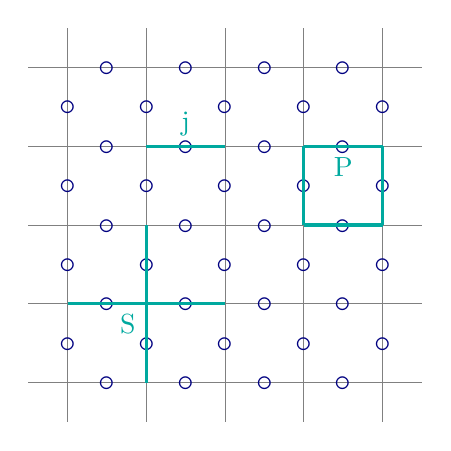
\begin{tikzpicture}
        \foreach \i in {1,...,5}
            \foreach \j in {1,...,5}{
                \draw[Gray] (\i,0.5) -- (\i,5.5);
                \draw[Gray] (0.5,\j) -- (5.5,\j);
            }
        \foreach \i in {1,...,4}
            \foreach \j in {1,...,5}{
                \node[NavyBlue, thick] at (\i+0.5,\j-0.02) {\large{$\mathbf{\circ}$}};
            }
        \foreach \i in {1,...,5}
            \foreach \j in {1,...,4}{
                \node[NavyBlue, thick] at (\i,\j+0.48) {\large{$\mathbf{\circ}$}};
            }
            \draw[very thick, Emerald] (2,4) -- (3,4) node[midway, above] {j};

            \draw[very thick, Emerald] (1,2) -- (3,2) node[midway, below left] {S};
            \draw[very thick, Emerald] (2,1) -- (2,3);

            \draw[very thick, Emerald] (4,4) -- (5,4) node[midway, below=0.25] {P};
            \draw[very thick, Emerald] (4,3) -- (5,3);
            \draw[very thick, Emerald] (5,3) -- (5,4);
            \draw[very thick, Emerald] (4,3) -- (4,4);

    \end{tikzpicture}}

    \caption[Figure showing a toric code lattice]{Figure showing a toric code lattice. Indicated are the spins (\textcolor{NavyBlue}{$\circ$}) and the bonds (j), stars (S) and plaquettes (P) used to describe the interactions.}
    \label{fig:toric_code}
\end{figure}

The states satisfying $A_s=1$ (for all $s$) must have vertices with even numbers of flipped spins (considering up spins as default and up spins as flipped). Therefore, the configurations of flipped spins must form closed loops, as 'drawn' by their corresponding bonds (see Figure \ref{fig:toric_code_loop}). For the possible configurations of loops, the action of $B_p$ stabilizer can either create further closed loops or deform the existing ones (without breaking or joining edges). The closed loops can be either trivial (can be contracted until disappearing) or non-trivial. Non-trivial loops wrap around the torus, and as such could not be contracted without 'snapping' their boundary line. There are then four distinct ground states as defined by loop configurations: trivial (equivalent to no loops), non-trivial loops in one of two possible directions in the torus, and a combination of the two non-trivial loops. These configurations cannot be deformed from one to another by A and B operations. Note how this degeneracy is directly linked to the topology of the torus.

\begin{figure}
    \centering
    \resizebox{0.45\textwidth}{!}{
    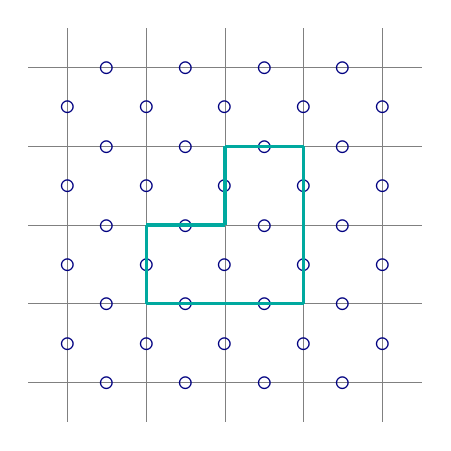
\begin{tikzpicture}
        \foreach \i in {1,...,5}
            \foreach \j in {1,...,5}{
                \draw[Gray] (\i,0.5) -- (\i,5.5);
                \draw[Gray] (0.5,\j) -- (5.5,\j);
            }
        \foreach \i in {1,...,4}
            \foreach \j in {1,...,5}{
                \node[NavyBlue, thick] at (\i+0.5,\j-0.02) {\large{$\mathbf{\circ}$}};
            }
        \foreach \i in {1,...,5}
            \foreach \j in {1,...,4}{
                \node[NavyBlue, thick] at (\i,\j+0.48) {\large{$\mathbf{\circ}$}};
            }

            \draw[very thick, Emerald] (3,4) -- (4,4);
            \draw[very thick, Emerald] (2,2) -- (4,2);
            \draw[very thick, Emerald] (4,2) -- (4,4);
            \draw[very thick, Emerald] (2,2) -- (2,3);
            \draw[very thick, Emerald] (3,3) -- (3,4);
            \draw[very thick, Emerald] (2,3) -- (3,3);

    \end{tikzpicture}}

    \caption{Example of a closed loop formed by down-spin bonds}
    \label{fig:toric_code_loop}
\end{figure}

The two qubits of information stored by this code are not sensitive to small local perturbations, and therefore constitute a good candidate for fault-tolerant quantum memory. Furthermore, computations on the logical qubits are also constructable, by implementing logical operators given by strings and loops of X and Z operators. \textcolor{red}{add citation of \url{https://www.physics.rutgers.edu/grad/602/Lectures/JC_Presentations/0419/Intro_Toric_Code.pdf}}

\subsection{The Surface Code}

The surface code was inspired by this toric code, and takes advantage of the fact that this topology is not a requirement for the development of this kind of stabilizer code, which can in fact be placed in a plane lattice. In this case the physical qubits are classified into data qubits and measurement qubits. The measurement qubits are associated with X measures or Z measures (as given by eigenvalues of the stabilizer terms A  and B discussed previously) performed on the adjacent data qubits (see Figure \ref{fig:surface_code_loop}).

\begin{figure}
    \centering
    \resizebox{0.45\textwidth}{!}{
    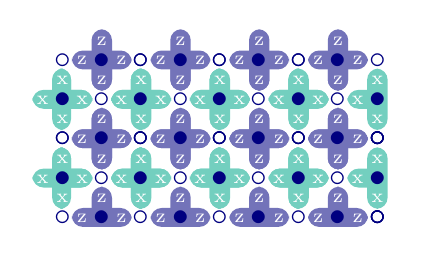
\begin{tikzpicture}
      
        \foreach \i in {1,...,4}
            \foreach \j in {1,...,2}{
                \ifthenelse{\i=1}{\fill[Emerald!55,thick,rounded corners]  (\i-0.1,\j+0.13) rectangle (\i+0.38,\j-0.11);
                \node[white] at (\i+0.25,\j) {\scriptsize{x}} ;}{\fill[Emerald!55,thick,rounded corners]  (\i-0.38,\j+0.13) rectangle (\i+0.38,\j-0.11);\node[White] at (\i-0.25,\j) {\scriptsize{x}} ;
                \node[white] at (\i+0.25,\j) {\scriptsize{x}} ;}
                
                \ifthenelse{\j=1}{\fill[Emerald!55,thick,rounded corners]  (\i-0.13,\j+0.4) rectangle (\i+0.11,\j-0.1);
                \node[White] at (\i,\j+0.25) {\scriptsize{x}} ;
                \fill[NavyBlue!55,thick,rounded corners]  (\i+0.5-0.38,\j+0.5+0.13-1) rectangle (\i+0.5+0.38,\j+0.5-0.11-1);\node[White] at (\i+0.25,\j+0.5-1) {\scriptsize{z}} ;
                \node[white] at (\i+0.75,\j+0.5-1) {\scriptsize{z}} ;
                \fill[NavyBlue!55,thick,rounded corners]  (\i+0.5-0.13,\j+0.5+0.4-1) rectangle (\i+0.5+0.13,\j+0.5-0.1-1); \node[White] at (\i+0.5,\j-0.25) {\scriptsize{z}};
                \node[NavyBlue, thick] at (\i,\j+0.5-1) {\large{$\mathbf{\circ}$}};
                \node[NavyBlue, thick] at (\i+0.5,\j+0.5-1) {\large{$\mathbf{\bullet}$}};
                \node[NavyBlue, thick] at (5,\j+0.5-1) {\large{$\mathbf{\circ}$}};
                }{}
                
                \fill[Emerald!55,thick,rounded corners]  (\i-0.13,\j+0.4) rectangle (\i+0.11,\j-0.38); \node[White] at (\i,\j-0.25) {\scriptsize{x}} ;
                \node[White] at (\i,\j+0.25) {\scriptsize{x}} ;

                \ifthenelse{\i=4}{
                \fill[Emerald!55,thick,rounded corners]  (\i+1-0.13,\j+0.4) rectangle (\i+1+0.13,\j-0.38); \node[White] at (\i+1,\j-0.25) {\scriptsize{x}} ; 

                \fill[Emerald!55,thick,rounded corners]  (\i-0.38+1,\j+0.13) rectangle (\i+1+0.1,\j-0.11);
                \node[white] at (\i+1-0.25,\j) {\scriptsize{x}} ;
                \node[White] at (\i+1,\j+0.25) {\scriptsize{x}} ;
                \node[NavyBlue, thick] at (\i+1,\j) {\large{$\mathbf{\bullet}$}};
                \node[NavyBlue, thick] at (\i+1,\j+0.5) {\large{$\mathbf{\circ}$}};}{}
                \fill[NavyBlue!55,thick,rounded corners]  (\i+0.5-0.38,\j+0.5+0.13) rectangle (\i+0.5+0.38,\j+0.5-0.11);\node[White] at (\i+0.25,\j+0.5) {\scriptsize{z}} ;
                \node[white] at (\i+0.75,\j+0.5) {\scriptsize{z}} ;


                \ifthenelse{\j=2}{\fill[NavyBlue!55,thick,rounded corners]  (\i+0.5-0.13,\j+0.5+0.1) rectangle (\i+0.5+0.13,\j+0.5-0.38); \node[White] at (\i+0.5,\j+0.25) {\scriptsize{z}};}{\fill[NavyBlue!55,thick,rounded corners]  (\i+0.5-0.13,\j+0.5+0.4) rectangle (\i+0.5+0.13,\j+0.5-0.38);\node[White] at (\i+0.5,\j+0.25) {\scriptsize{z}} ; \node[White] at (\i+0.5,\j+0.75) {\scriptsize{z}} ;}


                \node[NavyBlue, thick] at (\i+0.5,\j) {\large{$\mathbf{\circ}$}};
                \node[NavyBlue, thick] at (\i,\j) {\large{$\mathbf{\bullet}$}};
                \node[NavyBlue, thick] at (\i,\j+0.5) {\large{$\mathbf{\circ}$}};
                \node[NavyBlue, thick] at (\i+0.5,\j+0.5) {\large{$\mathbf{\bullet}$}};
            }
            

    \end{tikzpicture}}

    \caption[Surface code diagram]{Surface code diagram where measurement qubits are depicted by \textcolor{NavyBlue}{$\bullet$} and data qubits by \textcolor{NavyBlue}{$\circ$}. The four-qubit stabilizer measurements corresponding to each of them (X or Z) are also shown.}
    \label{fig:surface_code_loop}
\end{figure}

The code is executed as a series of cycles consisting of CNOT gate applications followed by projective measurements. The measurement qubits are first initialized to some ground state $\ket{g}$. For the Z measurement, the CNOT gates have the data qubits as control and the measurement qubit as the target, as shown in Figure \ref{fig:Zmeasurecycle}.

\begin{figure}
    \centering
    \begin{tikzpicture}
    \node[scale=1] {
    \begin{quantikz}
        \lstick{$\scriptstyle\ket{g}$} & \targ{} & \targ{} & \targ{} & \targ{} & \meter{}&\rstick[5]{$\scriptstyle\ket{\psi}_Z$}\\
        \lstick{$\scriptstyle a$}& \ctrl{-1} & & & & &\\
        \lstick{$\scriptstyle b$}& & \ctrl{-2} & & & &\\
        \lstick{$\scriptstyle c$}& & & \ctrl{-3} & & & \\
        \lstick{$\scriptstyle d$}& & & & \ctrl{-4} & & 
    \end{quantikz}};
    \end{tikzpicture}
    \caption[Z-measure cycle for the surface code]{Z-measure cycle for the surface code. The labels a, b, c and d refer to the four data quits adjacent to the measurement qubit}
    \label{fig:Zmeasurecycle}
\end{figure}
This cycle results in an eigenstate $\ket{\psi_Z}$ of the operation $Z_aZ_bZ_cZ_d$ with eigenvalues $\pm 1$.

Similarly, the X measure cycle applies the CNOT gate with the measure qubit as control, with the addition of Hadamard gates ($H$) before and after the CNOT operations. The cycle is shown in Figure \ref{fig:Xmeasurecycle}. Hadamard gates operations take the following matrix form:
\begin{equation}
    H=\cfrac{1}{\sqrt{2}}\begin{bmatrix}
        1&1\\
        1&-1
    \end{bmatrix}.
\end{equation}
The Hadamard gate is widely used in quantum computing algorithms, as it can be applied to initialize equiprobable superposition states from states $\ket{0}$ and $\ket{1}$. It can also be used to perform basis changes and to perform $X$ measurements using a Z gate by performing $HZH=X$.
\begin{figure}
    \centering
    \begin{tikzpicture}
    \node[scale=1] {
    \begin{quantikz}
        \lstick{$\scriptstyle\ket{g}$} & \gate{H}& \ctrl{1} & \ctrl{2} & \ctrl{3} & \ctrl{4} & \gate{H}& \meter{}&\rstick[5]{$\scriptstyle\ket{\psi}_X$}\\
        \lstick{$\scriptstyle a$}& &\targ & & & & & & &\\
        \lstick{$\scriptstyle b$}& & & \targ & & & & & &\\
        \lstick{$\scriptstyle c$}& & & & \targ & & & & &\\
        \lstick{$\scriptstyle d$}& & & & & \targ & & & &
    \end{quantikz}};
    \end{tikzpicture}
    \caption[X-measure cycle for the surface code]{X-measure cycle for the surface code. The labels a, b, c and d refer to the four data quits adjacent to the measurement qubit}
    \label{fig:Xmeasurecycle}
\end{figure}
The combined operations on an X measurement cycle produce an eigenstate $\ket{\psi_X}$ of $X_aX_bX_cX_d$ with eigenvalues $\pm 1$.

Performing a complete surface code cycle puts the system in a randomly selected \textit{quiescent state} $\ket{\psi}$. This state, as well as the outcomes $\pm 1$ of the stabilizer measurements, will be preserved in subsequent cycles (unless errors occur). The number of possible quiescent states is given by the lattice size, specifically by the number of measurement qubits $N$, scaling as $2^N$.

Consider what happens if a single-qubit error occurs. As an example, the error could be a phase flip acting on data qubit $a$. The deviation occurs with some small probability amplitude $\epsilon$ and is represented by operation $I_a+\epsilon Z_a$. The new state of the system is
\begin{equation}
    \ket{\psi'}=(I_a+\epsilon Z_a)\ket{\psi}.
\end{equation}
A subsequent measurement cycle will project this state into eigenstates of $Z_aZ_bZ_cZ_d$ and $X_aX_bX_cX_d$ once again. This will be highly likely to return the system to its prior state. However, there is a probability $\epsilon^2$ that after the cycle the state will be $Z_a\ket{\psi}$. This error will result in the modification of measurement qubit outcomes. Particularly, observe that there will be a sign change in the eigenvalue of $X_aX_bX_cX_d$:
\begin{equation}
    X_aX_bX_cX_d(Z_a\ket{\psi})=-Z_a(X_aX_bX_cX_d\ket{\psi})=-X_{abcd} Z_a\ket{\psi}
\end{equation}
where $X_{abcd}$ is the eigenvalue of $X_aX_bX_cX_d$ for quiescent state $\ket{\psi}$. The first step in the equation uses the anticommutativity of $Z_a$ and $X_a$ ($\{X_a,Z_a\}=X_aZ_a+Z_aX_a=0$)\footnote{The operator $Z_a$ also commutes with $X_b$, $X_c$ and $X_d$ as it acts on a different qubit.} Thus, the new state is also an eigenstate of the X stabilizer, with the opposite sign eigenvalue. The Z measurements surrounding the erroneous data qubit are unmodified due to $Z_a$ commuting with itself.

As the sign change affects both X measures surrounding the flipped data qubit, it is possible to identify which of the qubits suffered an error. Similarly, a bit-flip will be reflected in the outcomes of both adjacent Z measures. The repeated application of the cycles is also capable of detecting measurement errors. These could manifest, for example, a single sign change detected at a single measurement qubit (instead of two as related to the flips in data qubits). These errors will often disappear in later iterations of the cycle. If the errors are too likely, it becomes difficult to properly identify their cause, as proper identification requires them to be separated in space. If a misdiagnosed error gets corrected, it might lead to erroneous conclusions.

\subsection{Logical encodings on the surface code}

As can be seen in Figure \ref{fig:surface_code_loop}, surface codes are typically defined with \textit{rough} top and bottom boundaries given by measure-Z qubits, and \textit{smooth} measure-X boundaries to the left and to the right. The degrees of freedom for this case will be given by $2N$ (for $N$ the number of measurement qubits) and $2(N+1)$ corresponding to the data qubits. Then, the linearly independent set of stabilizers introduces $2N$ constraints. Therefore, the code can store one logical qubit's worth of information. Logical $X$ and $Z$ operators can be defined to manipulate the state of this qubit, by switching between quiescent states. The rate of logical errors (misidentified by the correction algorithm) will increase with code \textit{distance}, the minimum number of physical qubit flip operators required to define the logical operators. The logical operators commute with all stabilizers and must span the full length of the array. Thus, larger arrays are less sensitive to errors. 

To perform useful calculations it is of interest to have more than one logical qubit encoded in a surface code array. This can be achieved by removing some of the constraints to obtain higher degrees of freedom. To this end, boundaries must be modified, for example by alternating X and Z boundaries. However, operators cannot connect equal-type sections of these boundaries, limiting the code's usability. A more fruitful approach is to create 'holes' in the array by switching off (i.e. not executing) some of the measurement qubits. Details on the resulting logical operators for this approach can be accessed in \textcolor{red}{cite \url{https://arxiv.org/pdf/1208.0928}}.

\subsection{Surface Code Implementation}

The distance-three surface code was implemented using Python and the Qiskit package of quantum computing tools. \textcolor{red}{Add code plots}

\section{Quantum Error Correction for Bosonic Modes}

As introduced in the previous chapter, bosonic systems are interesting due to their increased coherence times compared with superconducting transmon qubits. Bosonic modes can be implemented using microwaves in superconducting resonant cavities, characterized by large quality factors and therefore low rates of energy loss. The frequency of the oscillators is given by their geometry. As this geometry is rigid, the intrinsic decoherence rates for the oscillators are extremely low (at times negligible). 

Due to the even spacing of the harmonic oscillator's energy levels, transmon qubits are needed for universal control. Classical controls can only displace the oscillator in phase space, maintaining coherence. Therefore, the advantages of the bosonic systems are somewhat dampened by the need for ancilla transmon qubits for control purposes. An error of the control elements would lead to decoherence in the cavity which must be addressed by fault-tolerance protocols.

The error correction methodology discussed throughout this chapter is based on defining logical qubits, spanning larger Hilbert spaces than each of the physical qubits contained within them. A harmonic oscillator's Hilbert space is intrinsically larger than that of a two-level system. This can be leveraged in the construction of logical qubits, as the physical qubits in these logical states must be highly entangled.

A further advantage of microwave bosonic modes is that their error rates are low. Moreover, they are dominated by one error type: photon loss. There is also no need to identify the element that incurred the error, as all of them simply happen within the harmonic oscillator. Bosonic error correction codes thus require smaller Hilbert spaces than qubit error correction to preserve the same amount of information.

The larger Hilbert spaces can also lead to efficient encodings. For example, the 8 states given by three qubits can be thought to correspond to levels $\ket{0}$ to $\ket{6}$ as follows:
\begin{eqnarray}
    \ket{000} & \iff \ket{0} \qquad \quad \ket{001} & \iff \ket{1} \notag\\ 
    \ket{010} & \iff \ket{2} \qquad \quad \ket{011} & \iff \ket{3} \notag\\
    \ket{100} & \iff \ket{4} \qquad \quad \ket{101} & \iff \ket{5} \notag\\
    \ket{110} & \iff \ket{6} \qquad \quad \ket{111} & \iff \ket{7}.
\end{eqnarray}
This type of encoding, however, is extremely limited as the number of oscillator photons needed grows exponentially with the qubit number, and so does the rate of photon loss. Realistic bosonic codes typically leverage only the lower levels of a harmonic oscillator. Furthermore, a single photon decay could represent several highly correlated errors in the binary qubits (for example going from $\ket{10000}$ down to $\ket{01111}$), making error correction impracticable. Other encoding approaches can be carried out. In particular, it is useful to encode qubits in terms of phase differences between states. 

Some of the most relevant codes for bosonic error correction include Schrodinger's cat codes and Gottesman-Kitaev-Preskill (GKP) codes. A simple but illustrative example of error correction comes from binomial codes, also known as 'kitten' codes due to their codewords being similar (though smaller) to those of the cat codes. This code presents similar capabilities to that of a four-qubit amplitude damping code, however, it can be executed through one oscillator mode and requires only one stabilizer. This represents a Hilbert space dimensionality reduction from 16 to just 5. It also differs from the qubit code in that it has been proven experimentally to reach and exceed the break-even point for error correction.

A simple binomial code can be constructed using the following codewords:
\begin{eqnarray}
    \ket{0_L}&=\frac{1}{\sqrt{2}}(\ket{0}+\ket{4})\\
    \ket{1_L}&=\ket{2}.
\end{eqnarray}
The codewords both have an average of two excitations and are eigenstates $+ 1$ of a photon number parity operator. Thus a parity output of $-1$ indicates an error. The parity operator can be defined in terms of creation and loss operators $a^\dagger$ and $a$ as follows:
\begin{equation}
    P=e^{i\pi a^\dagger a}.
\end{equation}
The operator is a stabilizer because it anticommutes with the loss operator ($Pa=-aP$) and thus can detect the decay of one photon. Clearly, the stabilizer must be applied often enough to avoid the possibility of an even number of decays, which would be undetectable. 

A further benefit of the binomial approach is that, having one mode rather than several qubits, it simplifies the Kraus operator set. The resulting Kraus representation contains only two operators linked to the no error case ($K_0$) and to the loss of one photon ($K_1$). The code is known to satisfy the Knill-Laflamme conditions and unitary correction operations can be defined and applied to correct errors.

\subsection{GKP codes}

As mentioned previously, Gottesman-Kitaev-Preskill (GKP) bosonic codes constitute an important branch in bosonic mode QEC. Although proposed over two decades ago, recent research has made strides in the applicability of this methodology, increasing interest. The basic premise behind these codes is to work within a lattice in the oscillator phase space. Due to the quantum nature of the oscillator, the position and momentum operators do not commute. Therefore, translations in phase space around an adiabatic\footnote{Slow, smooth} transport loop introduce a geometric phase.

The GKP codespace is the $+1$ eigenspace of a pair of translation operators in phase space. The stabilizers $\hat{S}_1=\hat{T}(\mathbf{U})$ and $\hat{S}_2=\hat{T}(\mathbf{V})$ must obey:
\begin{equation}
    \frac{1}{h}\mathbf{V}^T\Omega\mathbf{U}=2,
\end{equation}
where $h$ refers to the Planck constant, and $\mathbf{U}$ and $\mathbf{V}$ are vectors of the form $(\Delta_x,\Delta_p)$ for displacements in phase space. Factor $\Omega$ is a symplectic form:
\begin{equation}
    \Omega=\begin{bmatrix}
        0 &+1\\
        -1& 0
    \end{bmatrix}.
\end{equation}
From these constraints, the resulting codespace contains two states. Although the eigenstates for these operators exist in a continuum, selecting the $+1$ eigenvalue imposes a strong constraint.

For a square lattice, the stabilizers are (using $\hslash=1$ convention):
\begin{eqnarray}
    \hat{S}_p&=e^{+i2\sqrt{\pi}\hat{x}}\\
    \hat{S}_x&=e^{-i2\sqrt{\pi}\hat{p}}.
\end{eqnarray}
The associated codespace is given by (a priori) infinitely squeezed, infinite-energy logical states\footnote{Clearly these states are unphysical. Experimental implementations of the GKP code use Gaussians with some finite width. As stabilizer measurement cycles take place these states get closer to the idealized, infinitely squeezed states.}.
\begin{eqnarray}
    \psi_0&=\sum_{n=-\infty}^{+\infty} \delta(x-(2n)\sqrt{\pi})\\
    \psi_1&=\sum_{n=-\infty}^{+\infty} \delta(x-(2n+1)\sqrt{\pi})
\end{eqnarray}
The phase space translations shown in Figure \textcolor{red}{add figure} $X_L$, $Y_L$ $Z_L$ form a representation of the Pauli matrices (obeying all the expected properties). Operations over these states are represented by Gaussians, performing actions such as \textit{squeezing} of the bosonic modes.

The main goal behind GKP codes was to correct small displacements such as those given by the Pauli group of translations. Over time it has been shown that they are actually capable of addressing more complex errors as well.
For displacement errors, the effect is a change in the phases of the stabilizers. These changes are diagnosed by using ancilla qubits and performing conditional stabilizer displacements. The phase kickback caused by an ancilla measurement provides the real and imaginary parts of the error syndromes $\ket{psi}\hat{S}_x\bra{\psi}$ and $\ket{psi}\hat{S}_p\bra{\psi}$ (for a system in state $\ket{\psi}$).

Recall that for qubits, the break-even point was referred to where the logical qubit lifetime matched that of the longest-lived physical qubit. In this case, break-even occurs when the longest-lasting oscillator encoding (given by the lowest photon number, and thus losing photons at the slowest rate) is outlived.
\textcolor{red}{add figs from the code}

\clearpage

General \cite{Girvin2021} \cite{Andersen2020} \cite{Gottesman2009} \cite{Roffe2019} \cite{devitt}

Specific Implementations \cite{Krinner2021} \cite{Chen2021} \cite{cleland2022}

Bosonic \cite{campagne2020} \cite{Lau2016} \cite{Chuang1997} \cite{Terhal2020} \cite{Blais2020} \cite{Hu2019} \cite{Michael2016} \cite{Grimsmo2021} \cite{Cai2021} \cite{Brady2023} \cite{lachance2023}